% Reuse accepted label-free artwork through vector viewports; no pixel editing.
\usepackage{graphicx}
\usetikzlibrary{arrows.meta,calc}
\tikzset{flow/.style={-{Stealth[length=1.6mm,width=1.1mm]},line width=.75pt},
 wirelabel/.style={fill=white,inner sep=1.2mm},
 every node/.style={font=\fontsize{9}{11}\selectfont,align=center,inner sep=1pt}}
% Arguments: source left/top/right/bottom pixels; destination left/bottom/width mm.
\newcommand{\artpiece}[7]{
 \pgfmathsetmacro{\pieceScale}{#7/((#3-#1)*.1)}
 \begin{scope}[shift={(#5,#6)},scale=\pieceScale,transform shape]
  \clip (0,0) rectangle ({(#3-#1)*.1},{(#4-#2)*.1});
  \node[anchor=south west,inner sep=0pt] at ({-#1*.1},{-(931-#4)*.1})
   {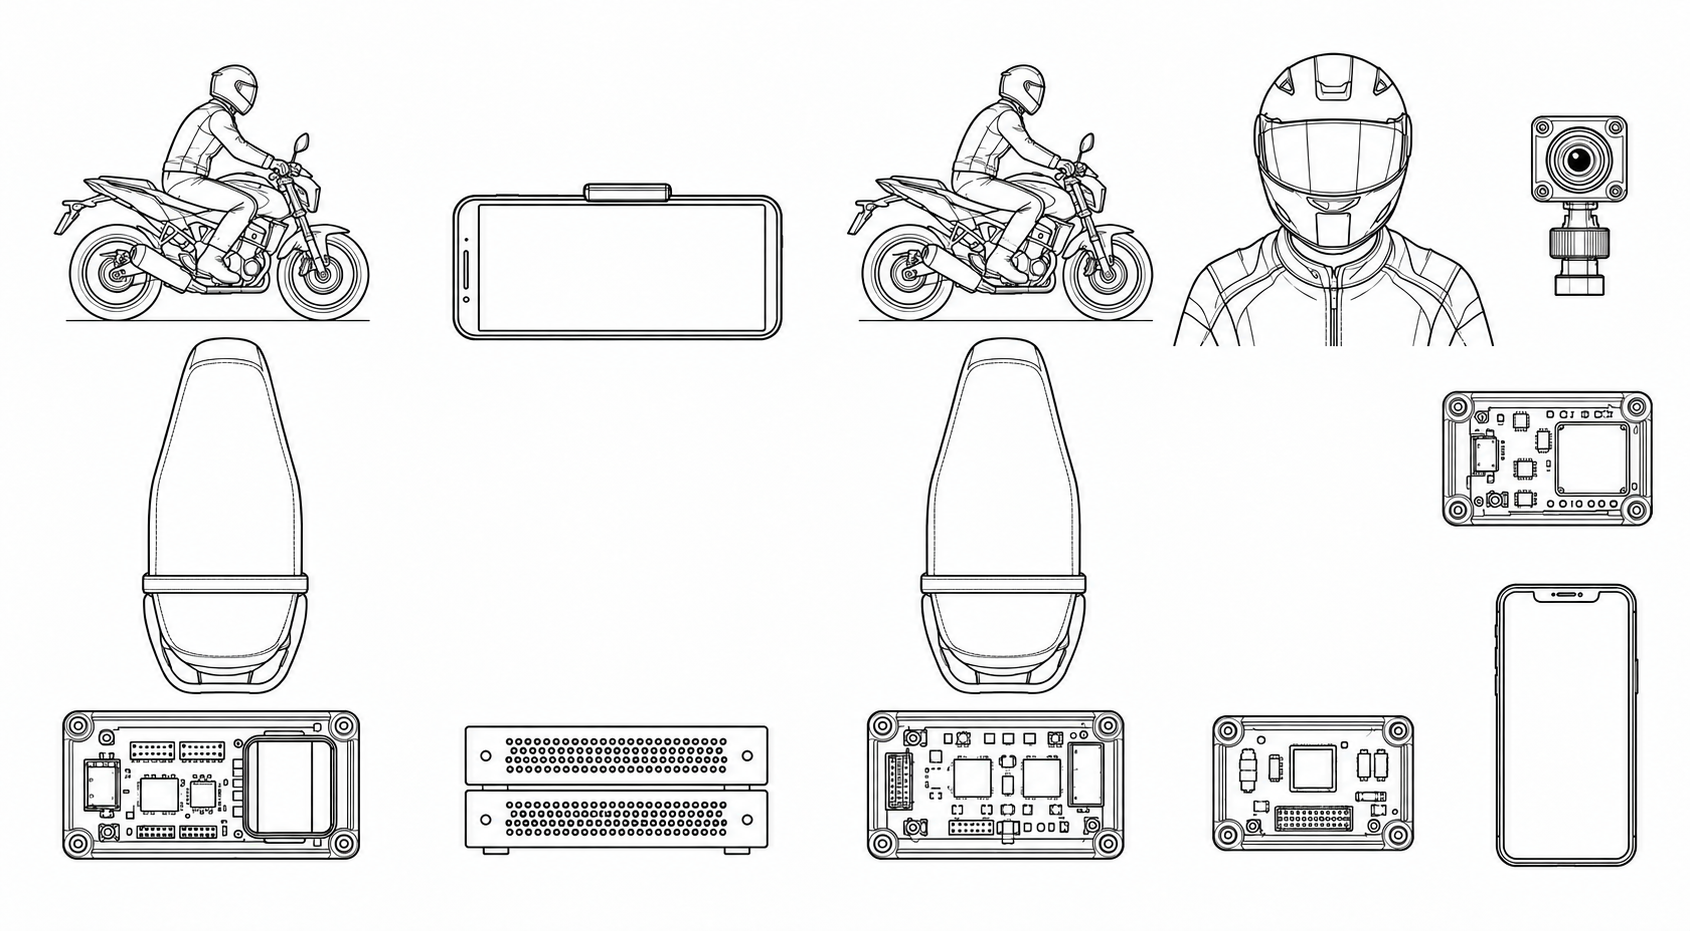
\includegraphics[width=169mm]{artwork-original.png}};
 \end{scope}}
\newcommand{\marker}[2]{
 \fill[white] (#1-2.4,#2-2.4) rectangle (#1+2.4,#2+2.4);
 \fill (#1-2,#2-2) rectangle (#1+2,#2+2);
 \fill[white] (#1-1.2,#2-1.2) rectangle (#1+1.2,#2+1.2);
 \fill (#1-1.2,#2-1.2) rectangle (#1,#2);
 \fill (#1,#2) rectangle (#1+1.2,#2+1.2);
}
\newcommand{\phoneglyph}[2]{
 \begin{scope}[shift={(#1,#2)}]
  \draw[densely dotted] (-8,0)--(8,0) (0,-13)--(0,13);
  \draw (0,10) .. controls (7,12) and (3,4) .. (7,-1)
    .. controls (11,-9) and (-4,-13) .. (-6,-7)
    .. controls (-9,0) and (-6,8) .. (0,10);
 \end{scope}}
